\cotefile{157-1}
\scanpage{98}

\mspage{104}

vertu de \uline{Der 3} $b'_1$ (ou seulement Der 3 $a'$).

\deleted{\uline{Définition} On dit que $f:X\to Y$ de $\mathrm{Diag}$ est une \uline{$\mathbb D$-fibration complète} si c'est une $\mathbb D$-fibrati-}

\uline{Prop. 4} On suppose que Der $a'$) est satisfait (\unsure{ou|où} toute $Z$ de $\mathrm{Diag}$ qui est Hot-asphérique, est \deleted{\unsure{totalement|complètement}}\inserted{complètement} $\mathbb D$-asphérique). Soit $f:X\to Y$ de $\mathrm{Diag}$. Les conditions suivantes sont équivalentes

$1^\circ)$ $f$ est une $\mathbb D$-fibration cohomologique \inserted{\uline{complète}} (conditions a) b) c) de \deleted{\unsure{la}}\unsure{définition|proposition} 2, page 101).

$2^\circ)$ Pour tout $F\in\mathrm{Ob}\,\mathbb D(X)$, loc \unsure{constant}, $f_*(F)$ \unsure{est} loc \unsure{constant}, se calcule fibre par fibre ; et Ça reste vrai après tout chgt. de base $Y'\to Y$ (avec $F'$, loc. const. sur $X'=X\times_Y Y'$). [Alors la formation de $f_*(F)$ commute à \uline{tout} chgt. de base.]

$3^\circ)$ Pour tout $Y''\overset{p}{\longrightarrow}Y'$, sur $Y$, si $p$ est une $\mathbb D$-équiv. coh. \deleted{alors}, alors $X''=X\times_Y Y''\to X'=X\times_Y\unsure{Y'|Y}$ aussi.

$3')$ Comme 3, \deleted{\unsure{en}} supposant que $Y''$ est la cat. ponctuelle, et que $Y'$ a \deleted{\unsure{un}} élément final : \deleted{\unsure{alors}} il faut que $X''\to X'$ soit une $\mathbb D$-équiv. coh.

% archive sheet number: 97
\scanpage{99}

\mspage{105}

\uline{Définition 3} : On dit que $f:X\to Y$ dans $\mathrm{Diag}$ est une $\mathbb D$-\uline{fibration complète} si c'est une $\mathbb D$-fibration cohomologique \inserted{complète} et une $\mathbb D$-fibration homologique \inserted{complète}.

C'est stable par chgt de base, par composition,

\deleted{\unsure{Comme} \unsure{corol.} : \unsure{les}}

La définition 3 équivaut à ceci : pour tout $p:Y''\to Y'$ sur $Y$, avec $Y''$ et $Y'$ Hot asphériques, le morphisme correspondant $X''\to X'$ est \uline{à la fois} une $\mathbb D$-équivalence cohomologique, et une $\mathbb D$-équivalence homologique. (Et il suffit \unsure{$=$} de le supposer pour $Y''=e$, et quand $Y'$ a un objet final ou un objet initial.) On peut songer à renforcer encore cette condition, en exigeant (sans regarder à gauche ni à droite) que $X''\to X'$ soit une \unsure{$\mathbb D$|$D$}-équivalence $1$-complète.

Mais il n'est pas clair que cette notion renforcée soit stable par composition -- à moins de la renforcer encore, en exigeant que si $Y''\to Y'$ est une $\mathbb D$-équiv. \unsure{$1$-complète|l-complète}, alors $X''\to X'$ l'est aussi. L'ennui avec cette définition renforcée, c'est que faute d'avoir une description cohomologique ou homologique de la \deleted{\unsure{coh.}}notion de

% archive sheet number: 98
\scanpage{100}

\mspage{106}

\margin{$\unsure{\ast|\times}$}

$\mathbb D$-équiv. $1$-complète, \deleted{\unsure{je}} on ne sera pas capable de donner des exemples intéressants (\unsure{i.e.} non \unsure{totalement} triviaux) de $\mathbb D$-fibrations en ce sens très fort. Sauf les Hot-fibrations triviales (\unsure{i.e.} à fibres Hot-asphériques) -- mais ce n'est pas drôle !

Mais quand on a des \inserted{produits $*$ \inserted{ass. et unit.} et des} $\mathcal H\mathrm{om}$ internes \inserted{correspondants} sur les $\mathbb D(X)_{\mathrm{loc.const.}}$, compatibles avec \margin{$\longrightarrow$}images inverses, \deleted{\unsure{et} tels que l'on ait}\inserted{\unsure{on a} pour $X$}, si $F$ et $G$ sont loc. \deleted{\unsure{$\mathrm{Hom}($}} const. dans $\mathbb D\unsure{(X)|eX)}$,

\[
\mathrm{Hom}(F,G)\simeq
\underbrace{\mathrm{Hom}\bigl(\underset{\substack{\vert\\\text{unité}\\\text{pour }*\\\text{dans }\mathbb D(X)}}{\unsure{\varepsilon|\xi}_X},\mathcal H\mathrm{om}(F,G)\bigr)}
_{\mathrm{Hom}(\underset{F}{\underline{\varepsilon_X*F}},G)}
\underset{\substack{\vert\\\text{car }\bar\varepsilon_{\unsure{A|X}}=p^*(\varepsilon_e)}}{\simeq}
\mathrm{Hom}_{\unsure{\mathcal A|A}}(\varepsilon_e,p_*\mathcal H\mathrm{om}(F,G)\unsure{)|\,}
\]

où $p:X\to e$, donc dans ce cas une \deleted{\unsure{$f$}}flèche $f:X\to Y$ de $\mathrm{Diag}$ est \deleted{\unsure{une}} $\mathbb D$-équiv. $1$-complète si (et seulement si) c'est une $\mathbb D$-équiv. coh.

Donc dans ce cas, \deleted{\unsure{la toute}} si $f$ est une $\mathbb D$-fib. cohomologique complète, c'est aussi une $\mathbb D$-\unsure{fib.} homologique complète, donc c'est une $\mathbb D$-fibration complète (déf. 3). (Et même au sens soi-disant renforcé de \deleted{\unsure{la|t}} \unsure{tantôt|tôtôt} : si $Y''\to Y'$ sur $Y$ est une $\mathbb D$-équiv. $1$-complète ($\Longleftrightarrow$ une $\mathbb D$-équiv. coh. !) alors $X''\to X'$ aussi.

% archive sheet number: 99
\scanpage{101}

\mspage{107}

Il se pose la question de trouver des $f$ qui soient des $\mathbb D$-fibrations cohomologiques, ou homologiques. Je ne sais si je serai capable d'en trouver, qui ne soient \unsure{pas} des HOT-fibrations cohomologiques, ou homologiques (cela revient maintenant au même$^*$), car pratiquement je ne sais \inserted{guère} dire qu'une flèche $Z'\to Z$ de $\mathrm{Cat}$ est une $\mathbb D$-équiv. coh. \inserted{complète}, que si cette flèche est une HOT-équivalence (et en admettant l'axiome Der 3 $b'_1$, ou sa variante affaiblie cohomologique).

% slanted
\margin{Car HOT-équiv. coh. $=$ HOT équiv. homol. $=$ HOT-équivalence, sans plus.}

Je vais \deleted{donc} chercher des HOT-fibrations, i.e. les $f:X\to Y$ tels que pour tout $Y''\to Y'\to Y$, avec $Y''$ et $Y'$ \deleted{\unsure{Hot}} asphériques (sous-entendu : pour HOT), $X''\to X'$ est une Hot-équivalence. \unsure{[}(Suffit \unsure{$=$} de supposer $Y''$ réduit à un point, $Y'$ avec objet final \ldots{}).

Supposons p. ex. $f$ propre (i.e. HOT-propre), \deleted{suffit} donc la condition a) de la \unsure{définition|proposition} 2, p. 107 satisfaite, et de \unsure{$=$} après tout chgt. de base. Suffit-il de vérifier de plus la condition b, i.e. que

\[
X_{/y}\longrightarrow X_{/y'},\quad \text{pour }y\to y'\text{ de }Y,
\]

sont des \deleted{\unsure{Hot-}}équivalences ? (J'entends, en restant sur $Y$, sans supposer aussi \inserted{d'avance} la \unsure{$=$} chose après changement de base.)

\deleted{Cela \deleted{\unsure{doit signifier}}\inserted{équivaut} \deleted{\unsure{sans}} donc à dire que $f_!(e_X)$ est loc. constant sur $\mathrm{HOT}(Y)$, et doit impliquer que $f_!(F)$ est loc. constant, dès que $F\in\mathrm{Ob}\,\mathrm{HOT}(X)$ l'est.}

% archive sheet number: 100
\scanpage{102}

\mspage{108}

Mais cela reste-il vrai après tout changement de base ?

La situation semble ici meilleure pour $f$ lisse (au lieu de propre), \deleted{alors} \inserted{en interprétant} les conditions a) et b) sous forme homologique, comme signifiant que $f_!(e_X)$ est un objet \uline{loc constant} de $\mathrm{HOT}(Y)$, qui se calcule fibre par fibre.

Comme $f$ lisse implique que $f_!$ commute à tout changement de base, \deleted{cette} cette hyp. \deleted{que $f$ \unsure{soit}} sur $f$ (que $f$ soit une HOT-fibration \deleted{\unsure{co}}homologique, peut-être pas complète) \deleted{implique} est stable par chgt de base, donc implique que c'est une HOT fibration cohomologique complète.

Mais cet argument utilise \deleted{des \unsure{opérations}} des propriétés générales des dérivateurs pour HOT, que je n'ai pas encore établies -- surtout pas dans le domaine $\mathrm{Cat}$ tout entier ! Donc il est sain de se méfier. Je préfère tâter la difficulté, en restant d'abord dans le cadre des \unsure{questions|prénotions|propriétés|opérations} \uline{cohomologiques} (\unsure{au moins|au mouv.}), dont j'ai une certaine maîtrise. Je suppose un $f$ propre encore, et \deleted{les conditions}\inserted{que les}

\[
X_y\to X_{/y},\quad X_{/y}\to X_{/\unsure{y|y'}},
\]

% archive sheet number: 102
\scanpage{103}

\mspage{109}

\margin{$\unsure{\ast|\times}$}

soient des HOT-équivalences, je veux prouver la $=$ chose après tout chgt de base, ou encore que dans la situation

\diagram{\begin{tikzcd}[ampersand replacement=\&,column sep=large]
 X\arrow[d,dash,"f"'] \& X'\arrow[l,"q"']\arrow[d,dash,"f'"'] \& X''\arrow[l,"q'"']\arrow[d,dash,"f''"]\\
 Y \& Y'\arrow[l,"p"] \& Y''\arrow[l,"p'"]
\end{tikzcd}}

si $Y',Y''$ sont asphériques alors $q'$ est une Hot-équivalence. Si je veux l'établir par \unsure{critères|critère} \unsure{cohomologiques|cohomologique}, je dois commencer par prendre sur $X'$ un faisceau \unsure{d'|l'}\uline{\unsure{ens|un}}, loc \unsure{constant} \inserted{$F$}, et prouver que $\Gamma(X',F)\simeq\Gamma(X'',q'{}^*F)$. Comme ce faisceau ne provient pas de $X$, je suis ennuyé pour appliquer l'hyp. sur $f$, qui concerne \unsure{a|à} priori des faisceaux \inserted{\unsure{d'ensembles|d'ens.|disons}} sur $X$, ou sur les $X_{/y}$.

Mais on devrait avoir ceci :

% slanted
\margin{$\downarrow$ Attention, ici je \uline{perds} la distinction entre HOT-équivalence, et Hot-équivalence}

\uline{Lemme} Soit $X''\overset{f}{\longrightarrow}X'$. \inserted{Alors $f$} est une HOT-équivalence

\[
\text{i.e.}\quad \deleted{\mathrm{Hom}_{\unsure{\mathbb D(X'')|\mathbb D(X')}}}
H^{\unsure{\cdot|i}}_{\mathrm{HOT}}(X',a_{X'})\xrightarrow{\sim}
H^{\cdot}_{\unsure{\mathrm{Hot}|\mathrm{HOT}}}(X'',a_{X''})
\]

est \deleted{\unsure{ibos|isos|iso}} pour tout $a\in\mathrm{Hot}=\mathrm{HOT}(e)$, \deleted{\unsure{alors}}\inserted{ssi} $f$ est \deleted{\unsure{$=$}} \inserted{une Hot-équivalence, et alors $f$ est même} une HOT-équiv. $2$-complète (\unsure{1-}\inserted{\uline{complète et homologique}}) \unsure{disons} seulement de : HOT-équiv. \uline{cohomologique}),

% slanted
\margin{Est-ce vrai aussi pour les dérivateurs $\mathbb D$ ?}

i.e. pour \deleted{tout} \deleted{\unsure{$a$ loc}} $\unsure{\xi|\zeta}\in\mathbb D(X')$ \uline{loc. \unsure{constant}} sur $X'$, on a $H^{\cdot}_{\mathrm{HOT}}(X',\xi)\xrightarrow{\sim}H^{\cdot}_{\mathrm{HOT}}(X'',q'{}^*(\xi))$\unsure{$($|/}.

% archive sheet number: 103
\scanpage{104}

\mspage{110}

\margin{$\unsure{\ast|\times}$}

La première assertion doit résulter des formules

\[
\begin{aligned}
\deleted{\unsure{\mathrm{Hom}}}\qquad H^{\unsure{\cdot|i}}_{\mathrm{HOT}}(Z,a_Z)&\simeq\underline{\mathcal H\mathrm{om}}_{\mathrm{Hot}}(\mathrm{hot}(Z),a)\\
(\text{et aussi }\quad H_{\unsure{\cdot|i}}^{\mathrm{HOT}}(Z,\unsure{a|e}_{\unsure{Z|z}})&\simeq\mathrm{hot}(Z)\times a\quad ,
\end{aligned}
\]

\deleted{\unsure{prenant} le $\pi_0$}

donc : si $(**)\ \mathrm{hot}(X'')\xrightarrow{\sim}\mathrm{hot}(X')$ est iso, alors $H^{\cdot}_{\mathrm{Hot}}(X^{\unsure{'|''}},a_{X'})\longrightarrow H^{\cdot}_{\mathrm{HOT}}(X'',a_{X''})$ est iso, puisque

c'est déduit de $(*)$ en prenant $\underline{\mathcal H\mathrm{om}}_{\mathrm{Hot}}(\cdot,a)$. Inversement, si $(*)$ est tjrs iso, \deleted{par exp} \margin{$\longrightarrow$}exprimant les deux \unsure{mb's|mbres} comme des $\underline{\mathcal H\mathrm{om}}_{\mathrm{Hot}}$ et prenant les $\pi_0$, on trouve que

\[
\mathrm{Hom}_{\mathrm{Hot}}(\mathrm{hot}(X'),a)\xrightarrow{\sim}
\mathrm{Hom}_{\mathrm{Hot}}(\mathrm{hot}(X''),\unsure{\cdot|a})
\]

est iso pour tout $a$, donc $(**)$ est iso.

Mais le fait que ça implique que $f''$ soit une \inserted{HOT-}équiv. \deleted{\unsure{$\mathbb D$}} coh. complète, i.e. que la relation $(*)$ reste vraie pour un $\unsure{\xi|\zeta}\in\mathbb D(X')$ \uline{loc. \unsure{constant}} sur $X'$, me paraît une \deleted{chose} propriété délicate du dérivateur HOT, sur laquelle il me faudra revenir.

Donc le lemme est loin d'être établi, faute d'avoir seulement construit le dérivateur HOT, sans $=$ parler d'en établir des propriétés spéciales délicates ! Mais je n'ai aucune raison de douter du lemme, il fait partie \inserted{de la kyrielle} des intuitions de base que je \deleted{\unsure{avais}} dois \deleted{\unsure{à}} fonder solidement.

% archive sheet number: 104
\scanpage{105}

\mspage{111}

Le lemme implique qu'une \inserted{$\mathbb D=$}HOT-fibration \deleted{cohomologique} (au sens de la définition 2 page \deleted{\unsure{81}}\inserted{\unsure{101|103}} \deleted{\unsure{qui est de}} revue et corrigée à la page 96\unsure{,|-}97) est en fait déjà une HOT-fibration cohomologique et homologique complète. Or on a vu que si $f$ est \uline{propre}, $f$ est une $\unsure{\mathbb D|\mathrm{H}}$-fibration ssi les conditions équivalentes \uline{sur $Y$} (sans chgt. de base) sont satisfaites. Et dualement pour $f$ lisse :

\figure{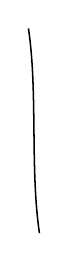
\begin{tikzpicture}[baseline]\draw[line width=.55pt] (0,2.6) .. controls (.12,1.8) and (.02,.8) .. (.14,0);\end{tikzpicture}}

\[
\searrow
\]

11.11.90

Je sens le besoin de réviser \deleted{\unsure{toutes}} les notions de $\mathbb D$-fibrations en tous genres \inserted{(p. \unsure{96|36} \unsure{ff|97})}. D'abord les diverses variantes utiles de l'axiome Der 3 sur les dérivateurs :

% slanted
\margin{Cf aussi la série \uline{Der} 3 c\unsure{\ldots} p. \unsure{114, 115|114--115}}

\uline{Der 3} a) si $Z\in\mathrm{Diag}$ est Hot-asphérique, il est $\mathbb D$-asphérique i.e. $\unsure{\mathcal A|A}=\mathbb D(e)\longrightarrow\mathbb D(Z)$ est pl. fidèle

a') Comme a), avec en plus la caractérisation de l'image essentielle de \deleted{\unsure{$\mathbb D$}} $\mathcal A$ dans $\mathbb D(Z)$, comme formée des $\mathbb D$-coeff. loc constants.

\uline{Der 3} b) Si $f:Z'\to Z$ de $\mathrm{Diag}$ est une Hot-équivalence, alors c'est une $\mathbb D$-équivalence, i.e. le foncteur $f^*:\mathbb D(Z)\to\mathbb D(Z')$ induit une \deleted{\unsure{fonction}}\inserted{équivalence} \deleted{pl. fidèle sur \unsure{la}} \inserted{entre les} sous-catégories formées des coefficients constants. (ou encore, un foncteur pl. fid $\mathbb D(Z)_{\mathrm{loc.const}}\longrightarrow\mathbb D(Z')$).

$b'_1)$ Si $f$ comme dessus, alors $f^{\unsure{\in|*}}$ est une $\mathbb D$-équivalence $1$-complète, i.e. le foncteur \deleted{\unsure{$f^*:\mathbb D(Z$}} $f^*:\mathbb D(Z)\to\mathbb D(Z')$ induit un foncteur pl fidèle

% archive sheet number: 105
\scanpage{106}

\mspage{112}

entre les sous-catégories pleines formées des objets loc. constants.

$b'_2)$ Comme $b'_1)$, mais avec $\mathbb D$-équiv. $2$-\uline{complète} au lieu de $1$-complète, i.e. $f^*$ induit une équivalence entre les sous-catégories formées des coeff. loc. const.

$b''_{\mathrm{coh}})$ Si $f:Z'\to Z$ de $\mathrm{Diag}$ est une Hot-équivalence, alors c'est une $\mathbb D$-équivalence cohomologique complète, i.e. pour tout $F\in\mathrm{Ob}\,\mathbb D(Z)$ qui est \uline{loc. constant},

\[
\text{on a}\qquad H^{\unsure{\cdot|i}}_{\mathbb D}(Z,F)\xrightarrow{\sim}H^{\cdot}_{\mathbb D}(Z',f^{\unsure{2|*}}F).
\]

$b''_{\mathrm{hom}})$ Si $f:Z'\to Z$ de $\mathrm{Diag}$ est une Hot-équivalence, c'est une $\mathbb D$-équivalence homologique complète, i.e. pour tout $F\in\mathrm{Ob}\,\mathbb D(Z)$ qui est \uline{loc. constant}, on a

\[
H_{\cdot}^{\mathbb D}(Z',f^*(F))\xrightarrow{\sim}H_{\cdot}^{\mathbb D}(Z,\unsure{F|E}).
\]

% slanted
\margin{Cf variantes $\pm$ spéciales pour HOT, pages \unsure{116 à 125|116/125}}

On a le diagramme d'implications tautologiques pour les variantes de Der 3 :

\diagram{\begin{tikzcd}[ampersand replacement=\&,column sep=small,row sep=small]
 \& b'_2\arrow[d,Rightarrow]\arrow[drr,Rightarrow] \& \& {}\\
 \& b'_1\arrow[dl,Rightarrow]\arrow[dr,Rightarrow]\arrow[dd,Rightarrow] \& \& a'\arrow[ddd,Rightarrow]\\
 b''_{\mathrm{coh}}\arrow[dr,Rightarrow] \& \& b''_{\mathrm{hom}}\arrow[dl,Rightarrow] \& {}\\
 \& b\arrow[drr,Rightarrow] \& \& {}\\
 \& \& \& a
\end{tikzcd}}

Dans tous les cas à ma connaissance, les dérivateurs satisfont la condition la plus forte Der 3 $b'_2$.

% archive sheet number: 106
\scanpage{107}

\mspage{113}

Je rappelle aussi la

\uline{Définition} 1 : Soit $f:\deleted{Z}X\to Y$ de $\mathrm{Diag}$. On dit que $f$ est une $\mathbb D$-\uline{équiv. cohomologique} (sous-entendu : ``\uline{complète}'') si pour tout $\mathbb D$-coeff. $F$ \uline{loc constant} sur $Y$,

\[
\deleted{\unsure{F|K}}\quad H^{\unsure{\cdot|i}}_{\mathbb D}(Y,F)\xrightarrow{\sim}H^{\cdot}_{\mathbb D}(X,f^{\unsure{\cdot|{\prime}|*}}F)\ ;
\]

on dit que $f$ est une $\mathbb D$-\uline{équivalence homologique} (``\uline{complète}'') si pour tout $F$ comme dessus,

\[
H_{\cdot}^{\mathbb D}(X,f^{\cdot}F)\xrightarrow{\sim}H_{\cdot}^{\mathbb D}(Y,F).
\]

On dit que $f$ est une $\mathbb D$-\uline{équivalence $1$-complète} (resp. $2$-\uline{complète}) si \deleted{pour} le foncteur

\[
f^*:\mathbb D(Y)_{\mathrm{loc.const.}}\longrightarrow\mathbb D(X)_{\mathrm{loc.const}}
\]

est pleinement fidèle (resp. une équivalence).

\diagram{\begin{tikzcd}[ampersand replacement=\&,row sep=small,column sep=small]
 \& \mathbb D\text{-équiv. }\unsure{2|3}\text{-complète}\arrow[d,Rightarrow] \& {}\\
 \& \mathbb D\text{-équiv. }1\text{-complète}\arrow[dl,Rightarrow]\arrow[dr,Rightarrow] \& {}\\
 \mathbb D\text{-équiv. coh.}\arrow[dr,Rightarrow] \& \& \mathbb D\text{-équiv. hom.}\arrow[dl,Rightarrow]\\
 \& \mathbb D\text{-équiv.} \&
\end{tikzcd}}

Si dans les \inserted{sous-catégories} $\mathbb D(X)_{\mathrm{loc.const}}$ il y a une loi $*$ (associative, unitaire, commutative) et des $\mathcal H\mathrm{om}$ internes associés, préservés par les images inverses, alors les $\mathbb D$-équiv. \deleted{$1$-complètes} cohomologiques sont déjà $1$-complètes, et sont \inserted{\unsure{bien|donc|même|aussi}} des $\mathbb D$-équiv. homologiques, donc dans ce cas particulier

% archive sheet number: 107
\scanpage{108}

\mspage{\handwritten{\unsure{114}}}\handwritten{\unsure{vide|v°}}

\mspage{\handwritten{117}}

Sans parler des \uline{cancéreux} qui font une métastase immédiatement après la vaccination (quand j'étais étudiante, le cancer était une contre-indication de la vaccination, elle ne l'est plus). Un de mes oncles parti en Afrique en pleine santé et réussite professionnelle pour un safari a dû subir toutes les vaccinations d'usage. Il est revenu épuisé et est mort dans l'année, de \deleted{leucémie.}

\deleted{Coïncidence ? Justement ça coïncide et c'est cette coïncidence que la science devrait expliquer.}

\deleted{Voici encore l'exemple de cette petite fille atteinte d'ipsa rythmie, guérie par un traitement cortisoné dans sa première enfance (maladie cérébrale entraînant idiotie et épilepsie). A 9 ans, le pédiatre déclare qu'on peut la vacciner ``puis qu'elle est guérie''. Depuis elle est épileptique. Elle a 16 ans.}

Coïncidence ? L'ennui c'est que cette coïncidence est fréquente dans l'épilepsie. J'en traite plusieurs cas qui se sont manifestés ``à l'âge des vaccinations''.

Et \unsure{cėtte|cètte|cette} petite fille vue à 6 mois se développant parfaitement bien cependant, qui débute une maladie de Little à 11 mois, aussitôt après la 1ère vaccination. Elle n'aura pas le tétanos, mais elle est paraplégique.

Coïncidence ? Justement ça coïncide étrangement et tant que l'on aura pas prouvé qu'il n'y a aucun lien entre la vaccination et la maladie qui ``coïncide'' comment obliger les parents à prendre ce risque.

Le 15 mai 1986, j'ai reçu une jeune femme pour troubles dépressifs, suite à la mort par encéphalite, 5 jours après une vaccination par le D.T.COQ, de son nourrisson de 4 mois. Cette vaccination ne faisait pas partie du lot retiré pour 48H. et l'accident n'a pas été communiqué à la presse.

\deleted{On ne convaincra jamais la maman qu'il ne s'agit que d'une coïncidence.}

\deleted{Est-ce une coïncidence aussi, ce que déclare le Dr.SARTORIUS de l'O.M.S. : ``On protège les enfants contre les maladies aigües, mais le nombre de maladies chroniques spécifiques s'accroit plus vite qu' l'ensemble de la popula\uuline{ti}on''.}

\deleted{Na-t-on pas le droit de choisir pour soi ou ses enfants entre le risque de maladie aigüe et le risque de maladie chronique ?}

\deleted{Ce même Dr. SARTORIUS nous dit encore : ``Pour les individus ayant vécu jusqu'à 65 ans, l'espérance de vie est de 75 ans dans les pays non médicalisés (le Nigéria par exemple) \deleted{comme} dans les pays d'Europe''.}

\deleted{Devons-nous donc être tellement fiers et sûrs de nos techniques au point de les imposer par l'obligation ?}

\deleted{Que l'on ne s'imagine pas que nous réclamons d'interdire les vaccinations ; les gens ont le droit de se protéger et protéger leurs enfants, ou leur chep}tel,des maladies aigües, par les vaccinations.

Ce que nous réclamons, et personnellement je le réclame à plusieurs titres :

- comme médecin homœopathe ayant à sa disposition une médecine prophylactique.

- comme française ayant hérité des valeurs de 1789.

- comme membre de l'A.C.A.T. luttant pour les droits de l'homme.

Ce que nous réclamons est très simple :

Que l'état laisse aux gens la liberté de choisir leur prophylaxie, même au risque de se tromper : ``errare humanum est'' et c'est sa grandeur. Et que ceux qui ont choisi la meilleure médecine soient récompensés par la meilleure santé qui leur servira de preuve.

\ldots/\ldots

\deleted{Voilà les faits que j'ai voulu résumer pour éclairer la Cour, sans l'ennuyer par de longs discours, au sujet du difficile problème que pose le procès de Monsieur COULARDEAU.}

\deleted{Ces faits parlent d'eux mêmes pour montrer que la médecine qu'a choisie Monsieur COULARDEAU pour garantir la santé de son troupeau vaut bien la facile vaccination et qu'en se donnant le mal de traiter ses bêtes par une thérapie individualisée il leur confère un degré de santé supérieure à celle qui est simplement requise par la loi au moyen des vaccinations. Je répéterai donc ce qu'ont signé mes 26 confrères homœopathes dans leur lettre à Monsieur le Préfet de la Haute-Loire : Monsieur COULARDEAU a satisfait à l'esprit de la loi plus que ceux qui satisfont à la lettre, et en attendant que soit réformé la lettre au nom de l'esprit qui l'a inspirée, nous espérons que Monsieur COULARDEAU sera jugé en fonction de cet esprit.}

\handwritten{\unsure{S Fayeton|A Fayeton|S. Fayeton}.}\\

% printed form
Docteur Simone FAYETON\\
01 - Généraliste \qquad Conventionné Hon. Lib.\\
Le Clos de Corsac\\
43700 BRIVES CHARENSAC\\
43 1 00308 6

\figure{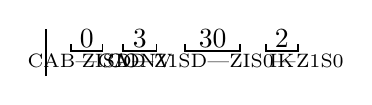
\begin{tikzpicture}[x=.66cm,y=.66cm,every node/.style={inner sep=0pt}]
\draw[line width=.8pt] (0,-.49)--(0,.42); \node at (.78,.24) {0}; \node at (1.80,.24) {3}; \node at (3.20,.24) {30}; \node at (4.53,.24) {2}; \draw[line width=.65pt] (.48,.12)--(.48,0)--(1.08,0)--(1.08,.12); \draw[line width=.65pt] (1.48,.12)--(1.48,0)--(2.12,0)--(2.12,.12); \draw[line width=.65pt] (2.67,.12)--(2.67,0)--(3.73,0)--(3.73,.12); \draw[line width=.65pt] (4.22,.12)--(4.22,0)--(4.84,0)--(4.84,.12); \node[font=\scriptsize] at (.78,-.20) {\unsure{CAB|CAD}}; \node[font=\scriptsize] at (1.80,-.20) {CONV}; \node[font=\scriptsize] at (3.20,-.20) {\unsure{ZISD|Z1SD|ZIS0|Z1S0}}; \node[font=\scriptsize] at (4.53,-.20) {IK};
\end{tikzpicture}}

% archive sheet number: 108
\scanpage{109}

\mspage{115}

\diagram{\begin{tikzcd}[ampersand replacement=\&,row sep=small]
 \mathbb D\text{-équiv. }2\text{-complète}\arrow[d,Rightarrow] \& {}\\
 \mathbb D\text{-}\unsure{\text{équi}|\text{équiv.}}\ 1\text{-complète}\arrow[r,Leftrightarrow] \& \mathbb D\text{-équiv. coh.}\arrow[d,Rightarrow]\\
 \& \mathbb D\text{-équiv. hom.}\arrow[d,Rightarrow]\\
 \& \mathbb D\text{-équivalence}
\end{tikzcd}}

Pour \deleted{\unsure{HOT}} $\mathbb D=\mathrm{HOT}$, toutes \unsure{les|ces} notions devraient être équivalentes, et équivalentes \deleted{en fait} à la condition encore plus faible en apparence, que $f:X\to Y$ soit une Hot-équivalence.

Mais je ne connais que HOT comme dérivateur où la $\mathbb D$-équivalence d'une flèche $f:X\to Y$ de $\mathrm{Diag}$ implique déjà la $\mathbb D$-équiv. coh. (complète), ou la $\mathbb D$-équivalence homologique (complète), voire même la $\mathbb D$-équivalence $1$-complète. (Je reviendrai là-dessus tantôt.)

\uline{Prop. 1} Soit $f:X\to Y$ de $\mathrm{Diag}$. Conditions équivalentes :

a) Pour tout $y\in\mathrm{Ob}\,Y$, l'inclusion $X_y\to X_{/y}$ est une $\mathbb D$-équiv., et pour toute flèche $y'\to y$ de $Y$, $X_{/y'}\to\unsure{X_{/y}|Y_{/y}}$ est une $\mathbb D$-équiv.

b) Pour tout \deleted{faisceau}\inserted{coeff.} \uline{constant} $F$ sur $Y$, $f_* f^* F$ est loc. constant, et se calcule ``fibre par fibre''.

(C'est la prop. 1 p. \unsure{76|75})

\uline{Prop. 1'} duale

% archive sheet number: 109
\scanpage{110}

\mspage{116}

\uline{Définition 2} Sous les conditions équivalentes de la \deleted{définition} prop. 1, on dit que $f$ est une $\mathbb D$\uline{-fibration cohomologique faible}. Sous les conditions duales, que $f$ est une $\mathbb D$\uline{-fibration homologique faible}.

C'est ce que dans la définition 1 p. 77 j'appelais ``$\mathbb D$-fibration cohomologique'' ou ``$\mathbb D$-fibration à gauche'', \inserted{et dualement.} Maintenant la notion me paraît trop faible pour mériter ce nom, que je réserve pour le cas ``complet''.

\uline{Prop 2} Les $\mathbb D$-fibrations coh. faibles sont stables par \unsure{changement|changements} de base lisses, les $\mathbb D$-fibr. hom. faibles stables par chang. de base propres.

Je devrais construire un exemple où \deleted{\unsure{on ait une}}\inserted{$f$ est une} $\mathbb D$-fibr. coh. faible, et ne l'est plus après chgt. de base.

\inserted{\uline{Prop. 3} \deleted{\unsure{Soit} $f:X\to Y$ de $\mathrm{Diag}$,} soit
\diagram{\begin{tikzcd}[ampersand replacement=\&,row sep=small,column sep=small]
 X\arrow[rr,"f"]\arrow[dr,"p"'] \& \& X'\arrow[dl,"p'"]\\
 \& S \&
\end{tikzcd}}
de $\mathrm{Diag}$, avec $p$ et $p'$ des $\mathbb D$-fibr. coh. faibles (resp. des $\mathbb D$-fibr. hom. faibles), soit $S_0\subset S$ tel que $\pi_0(S_0)\to\pi_0(S)$ surj. Pour que $f$ soit une $\mathbb D$-équiv., il suffit que \unsure{les} $f_s:X_s\to X'_s$, pour $s\in S_0$, le soient.}

\uline{Prop. 4} Si $f:X\to Y$ de $\mathrm{Diag}$ est $\mathbb D$-propre (resp. $\mathbb D$-lisse), alors $f$ est une $\mathbb D$-fibration coh. \deleted{faible} (resp. hom.) faible ssi pour tout $\unsure{F|E}$ constant sur $Y$, $f_* f^*F$ \inserted{(resp. $f_!f^*F$)} est loc. constant sur $Y$. Et s'il en est ainsi, \deleted{\unsure{D} cette condition est \unsure{co}} pour tout $Y'\to Y$ de $\mathrm{Diag}$, $f':X'=X\times_Y Y'\to Y'$ est encore une $\mathbb D$-fib. coh. (resp. hom.) faible.

\deleted{\unsure{En effet,}} Immédiat sur le critère b) de prop. 1.

% archive sheet number: 110
\scanpage{111}

\mspage{117}

\uline{Prop. 5} Soit $f:X\to Y$ de $\mathrm{Diag}$. Considérons les conditions suivantes :

a) Pour tout $Y''\to Y'$ sur $Y$ de $\mathrm{Diag}$, si $Y''$ et $Y'$ sont Hot-asphériques, alors

\[
X''=X\times_Y Y''\longrightarrow X\times_Y Y'
\]

est une $\mathbb D$-équivalence.

\diagram{\begin{tikzcd}[ampersand replacement=\&,column sep=small,row sep=small]
 X\arrow[d] \& X'\arrow[l]\arrow[d] \& X''\arrow[l]\arrow[d]\arrow[d,dash,start anchor=east,end anchor=south west,out=-55,in=22,looseness=1.55,shorten >=-5pt]\\
 Y \& Y'\arrow[l] \& Y''\arrow[l,"p"]
\end{tikzcd}}

a') Comme a), mais en supposant $p:Y''\to Y'$ une Hot-équiv. \inserted{(au lieu de supposer $Y',Y''$ \deleted{\unsure{$\mathbb D$}} Hot-asphériques)}

\deleted{\unsure{a'')} Comme a), mais en supposant $p:Y''\to Y'$ une $\mathbb D$-équiv. \unsure{1-complète}}

\deleted{\unsure{a'|a}}$a_1)$ Comme a), \deleted{\unsure{alors}} \unsure{en} supposant (au lieu de l'asphéricité) que $Y'$ a un objet final, et $Y''$ est la cat. unité.

$a^{\unsure{2|\,}}_2)$ Comme a), \deleted{\unsure{en}} mais en supposant que $Y'$ a un objet cofinal, et $Y''$ est la cat. unité.

$b_1)$ $f$ est une $\mathbb D$-fibration cohomologique faible, et le reste après tout changement de base.

$b_2)$ $f$ est une $\mathbb D$-fibration homologique faible, et le reste après tout chgt. de base.

On a alors le diagramme d'implications \inserted{tautologiques}

\diagram{\begin{tikzcd}[ampersand replacement=\&,row sep=small,column sep=small]
 \& \& a'\arrow[d,Rightarrow] \& \& {}\\
 \& \& a\arrow[dll,Rightarrow]\arrow[dl,Rightarrow]\arrow[drr,Rightarrow,shorten >=8pt]\arrow[drr,Rightarrow] \& \& {}\\
 a_1\arrow[r,Leftrightarrow] \& b_1 \& {} \& b_2\arrow[r,Leftrightarrow] \& a_2
\end{tikzcd}}

Lorsque $\mathbb D$ satisfait l'axiome Der 3 a' (p. 111), alors toutes ces conditions \inserted{sauf a')} sont équivalentes. \inserted{Lorsque $\mathbb D$ satisfait à l'axiome Der 3 $b'_1$ (ou seulement Der 3 $b''_{\mathrm{coh}}$ ou $b''_{\mathrm{hom}}$), alors toutes les conditions (y inclus a') sont équivalentes.} Pour simplifier, on va par la suite supposer que l'axiome Der 3 a') est satisfait.

\figure{\begin{tikzpicture}[x=0.4cm,y=0.4cm]\draw (0,0)--(-0.04,1.18);\end{tikzpicture}}
\uline{Définition} 3 : Sous les conditions équivalentes \inserted{$a,a_1,b_1,a_2,b_2$} de la prop. 4, on dit que $f$ est une $\mathbb D$-\uline{fibration}

% archive sheet number: 111
\scanpage{112}

\mspage{118}

\uline{Prop 6} Supposons que $f:X\longrightarrow Y$ de $\mathrm{Diag}$ soit \inserted{$\mathbb D$-}propre (resp. $\mathbb D$-lisse). \deleted{Alors $f$ est une $\mathbb D$-fibr. ssi c'est une $\mathbb D$-fibration coh. \deleted{\unsure{fa}} (resp. hom.) faible, ou encore} \inserted{Conditions équivalentes}

a) $f$ est une $\mathbb D$-fib. \unsure{(resp.}

b) $f$ est une $\mathbb D$-fibr. coh. (resp. hom) faible

c) $\forall\,y'\longrightarrow y$ de $Y$, $X_{/y'}\longrightarrow X_{/y}$ (resp. $\,{}_{y\backslash}X_{\deleted{\unsure{y}}}\longrightarrow{}_{y'\backslash}X$) est une $\mathbb D$-équivalence

d) $\forall\,F$ constant sur $Y$, $f_*f^*F$ (resp. $f_!f^*F$) est loc. constant sur $Y$

d') $\forall\,F$ loc constant sur $Y$, $f_*f^*F$ (resp $f_!f^*F$) est loc. constant sur $Y$.

Cela résulte formellement des Prop. 4 et Prop. 5.

\inserted{\uline{Cor.} Supposons $f:X\longrightarrow Y$ Cat-fibrant (resp. Cat-cofibrant). Pour que $f$ soit une $\mathbb D$-fibration, il f. et s. que \deleted{\unsure{les}} pour
% margin note written sideways
tout $u:y\longrightarrow y'$ de $Y$, $u^*:X_{y'}\longrightarrow X_y$ (resp. $u_*:X_y\longrightarrow X_{y'}$) soit une $\mathbb D$-équivalence}

\margin{\figure{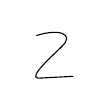
\begin{tikzpicture}[x=0.47cm,y=0.47cm]\draw (0,1.2) .. controls (.6,1.4) and (1.05,1.25) .. (.69,.91) .. controls (.43,.65) and (-.22,.08) .. (.04,.05) -- (1.0,.1);\end{tikzpicture}}}
Il est immédiat que la notion de $\mathbb D$-fibration est stable par chgt. de base, mais il est douteux qu'elle le soit par composition. (Ici encore, \unsure{je pourrais|je devrais|on pourrait} \unsure{ds l'immédiat} faire un contre-exemple, avec $\mathbb D\deleted{\unsure{=k}}=\mathrm{Der}(k\text{-}\mathrm{Mod})$ disons.)

% slanted
\margin{\uline{NB} Si les $\mathbb D$-équivalences sont déjà des Hot-équivalences, alors la notion \unsure{coïncide} avec celle des Hot-fibrations, et elle est stable par composition. \unsure{Égdemt|Égalemt}, si les $\mathbb D$-équivalences sont des $\mathbb D$-équivlc. coh., \unsure{ou} homologiques, alors la notion coïncide resp. avec celle des $\mathbb D$-fibrations cohomologiques (resp. homologiques), ci-dessus. et elle est également stable par \unsure{compos.|composition}}

Autre lacune de la notion : il n'est pas clair, si $f$\inserted{$:X\longrightarrow Y$} est une $\mathbb D$-fibration et $F$ un \deleted{\unsure{$\xi$|$f$}} $\mathbb D$-coeff. sur $Y$, si \deleted{\unsure{$\xi$|$f$}}

\[ f_*f^*F\qquad\text{et}\qquad f_!f^*F \]

se calculent ``fibre par fibre'', comme on attendrait dans le cas d'une ``fibré''.

Par contre, voici un résultat sympa :

% archive sheet number: 112
\scanpage{113}

\mspage{119}
\margin{$\unsure{\times|\ast}$}

\uline{Prop. \deleted{\unsure{6}}7} Soit $f:X\longrightarrow Y$ dans $\mathrm{Diag}$. Conditions équivalentes :

a) $f$ est une $\mathbb D$-équivalence ``universelle'', i.e. pour tout $Y'\longrightarrow Y$ de $\mathrm{Diag}$, $f':X'=X\times_Y Y'\longrightarrow Y'$ est une $\mathbb D$-équivalence.

b) $f$ est une $\mathbb D$-fibration à fibres $\mathbb D$-asphériques.

\uline{Définition 4} Sous les conditions équivalentes de la prop. 6, on dit que $f$ est une $\mathbb D$-fibration \uline{triviale}.

\margin{\figure{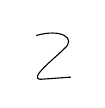
\begin{tikzpicture}[x=0.46cm,y=0.46cm]\draw (0,1.25) .. controls (0.7,1.45) and (1.12,1.17) .. (0.77,0.88) .. controls (0.5,0.61) and (-0.22,0.06) .. (0.12,0.04) -- (0.96,0.1);\end{tikzpicture}}}

Mais attention, $f$ peut-être une $\mathbb D$-fibration et une $\mathbb D$-équivalence, sans que la $\mathbb D$-fibration soit triviale i.e. sans que les fibres soient $\mathbb D$-asphériques, cf p. \unsure{87|85} ff. Et \unsure{ici même|certainement|sûrement} (devrais \unsure{remontrer|remonter}) même si $\mathbb D$ satisfait $\mathrm{Der}\,3\,b_2$ (la plus forte des variantes de $\mathrm{Der}\,3$), donc quand \uline{toutes} les conditions de la prop. 5, y inclus a'), sont équivalentes, celles-ci (i.e. que $f$ soit une $\mathbb D$-fibration) n'impliquent pourtant pas, en général, que dans la condition a') on puisse se borner à $p:Y''\longrightarrow Y'$ une $\mathbb D$-équivalence (au lieu d'une Hot-équivalence) : En d'autres termes, si on a un diagramme cartésien dans $\mathrm{Diag}$

\margin{\figure{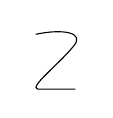
\begin{tikzpicture}[x=0.48cm,y=0.48cm]\draw (0,1.52) .. controls (0.76,1.68) and (1.29,1.55) .. (1.01,1.22) .. controls (0.64,0.75) and (-0.20,0.11) .. (0.05,0.07) -- (1.05,0.07);\end{tikzpicture}}}

\diagram{\begin{tikzcd}[ampersand replacement=\&,row sep=small,column sep=small]
X \arrow[d,"f"'] \& X' \arrow[l,"q"'] \arrow[d,"f'"]\\
Y \& Y' \arrow[l,"p"]
\end{tikzcd}},

avec $f$ une $\mathbb D$-fibration, et $p$ une $\mathbb D$-équivalence, \unsure{il|et} \unsure{ne|on} s'ensuit pas forcément que $q$ soit une $\mathbb D$-équivalence. (Mais ce sera pourtant le cas, \inserted{au moins} si $\mathbb D=\mathrm{HOT}$)

% archive sheet number: 113
